\section{Aufgabenanalyse}

\subsection{Systemvoraussetzungen}
Unser System ist in sich geschlossen. Einzig für die Kommunikation mit dem Arduino werden wir uns einer App bedienen, die als User-Interface dienen soll. Auch soll das System Akkubetrieben sein, was einen vollen Akku und dementsprechend ein passendes Ladegerät voraussetzen.

\subsection{Problemdefinition}
Das schwere Schleppen von einer Kühlbox, soll mithilfe eines mechatronischen Systems erleichtert werden. Die Idee war, die Schlepparbeit vom Auto zu einem Ort, an dem man sich mit der Familie oder mit Freunden niederlässt, etwas leichter zu gestalten. Dies soll auch als Problemlösung für Personen dienen, die nicht mehr schwere Dinge tragen dürfen oder können. Dabei soll auf etwas Lustiges und Nützliches zurückgegriffen werden können.

\subsection{Systemabgernzung}
Um die Aufgaben für das Projekt einzugrenzen und eine Übersicht über die zu erreichenden Punkte zu erhalten, wurde eine Systemabgrenzung, zur von uns selbst gestellten Aufgabenstellung, erstellt. Diese Systemabgrenzung, angefangen mit dem Umsystem nach den PESTEL-Guidelines zeigt an sich weder Details noch Unerwartetes auf:

\begin{figure}[H]
    \begin{center}
    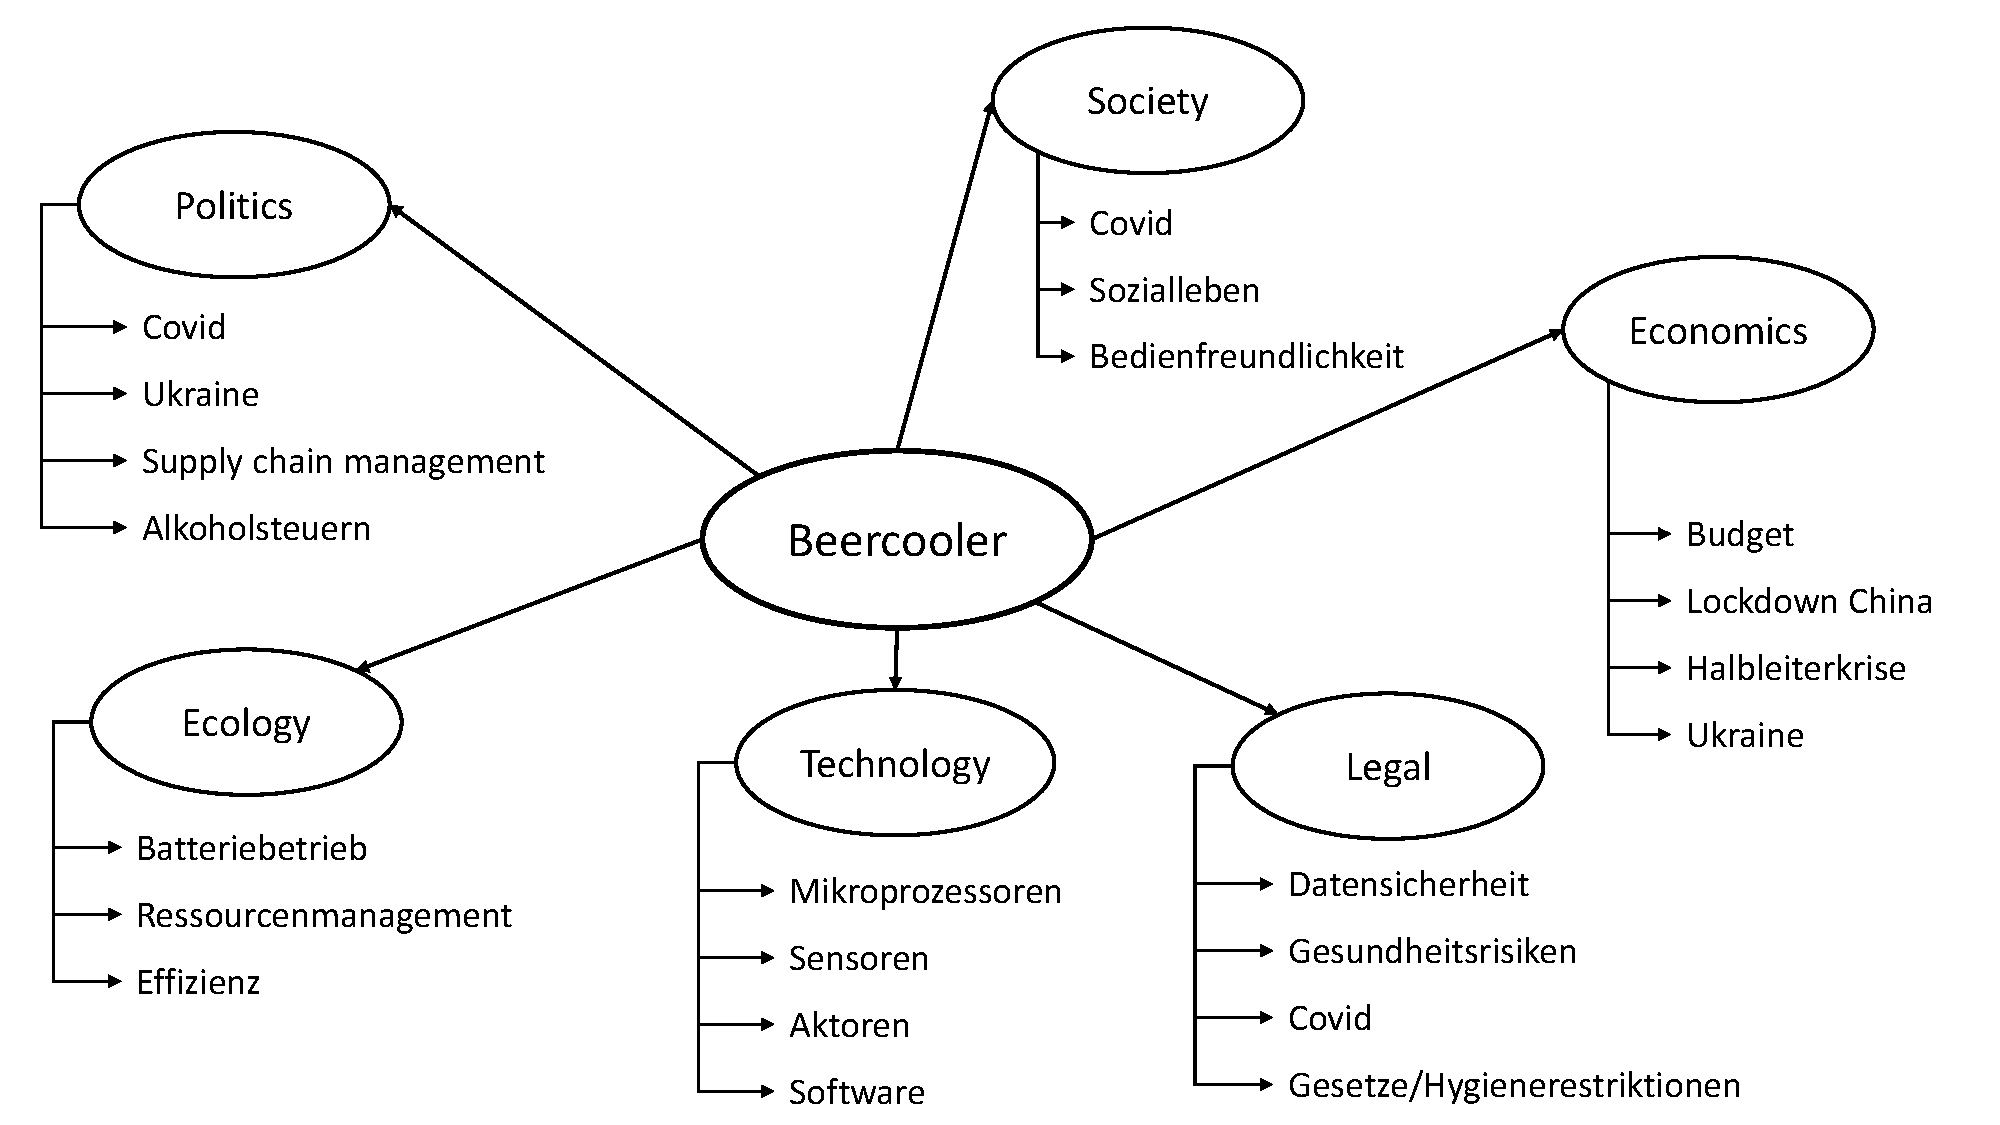
\includegraphics[width=\linewidth]{pestel.pdf}
    \end{center}
    \caption{Umfeld der Systemabgrenzung nach PESTEL}
\end{figure}

Bei genauerer Betrachtung des Umsystem kommt bereits etwas mehr zum Vorschein:

\begin{figure}[H]
    \begin{center}
    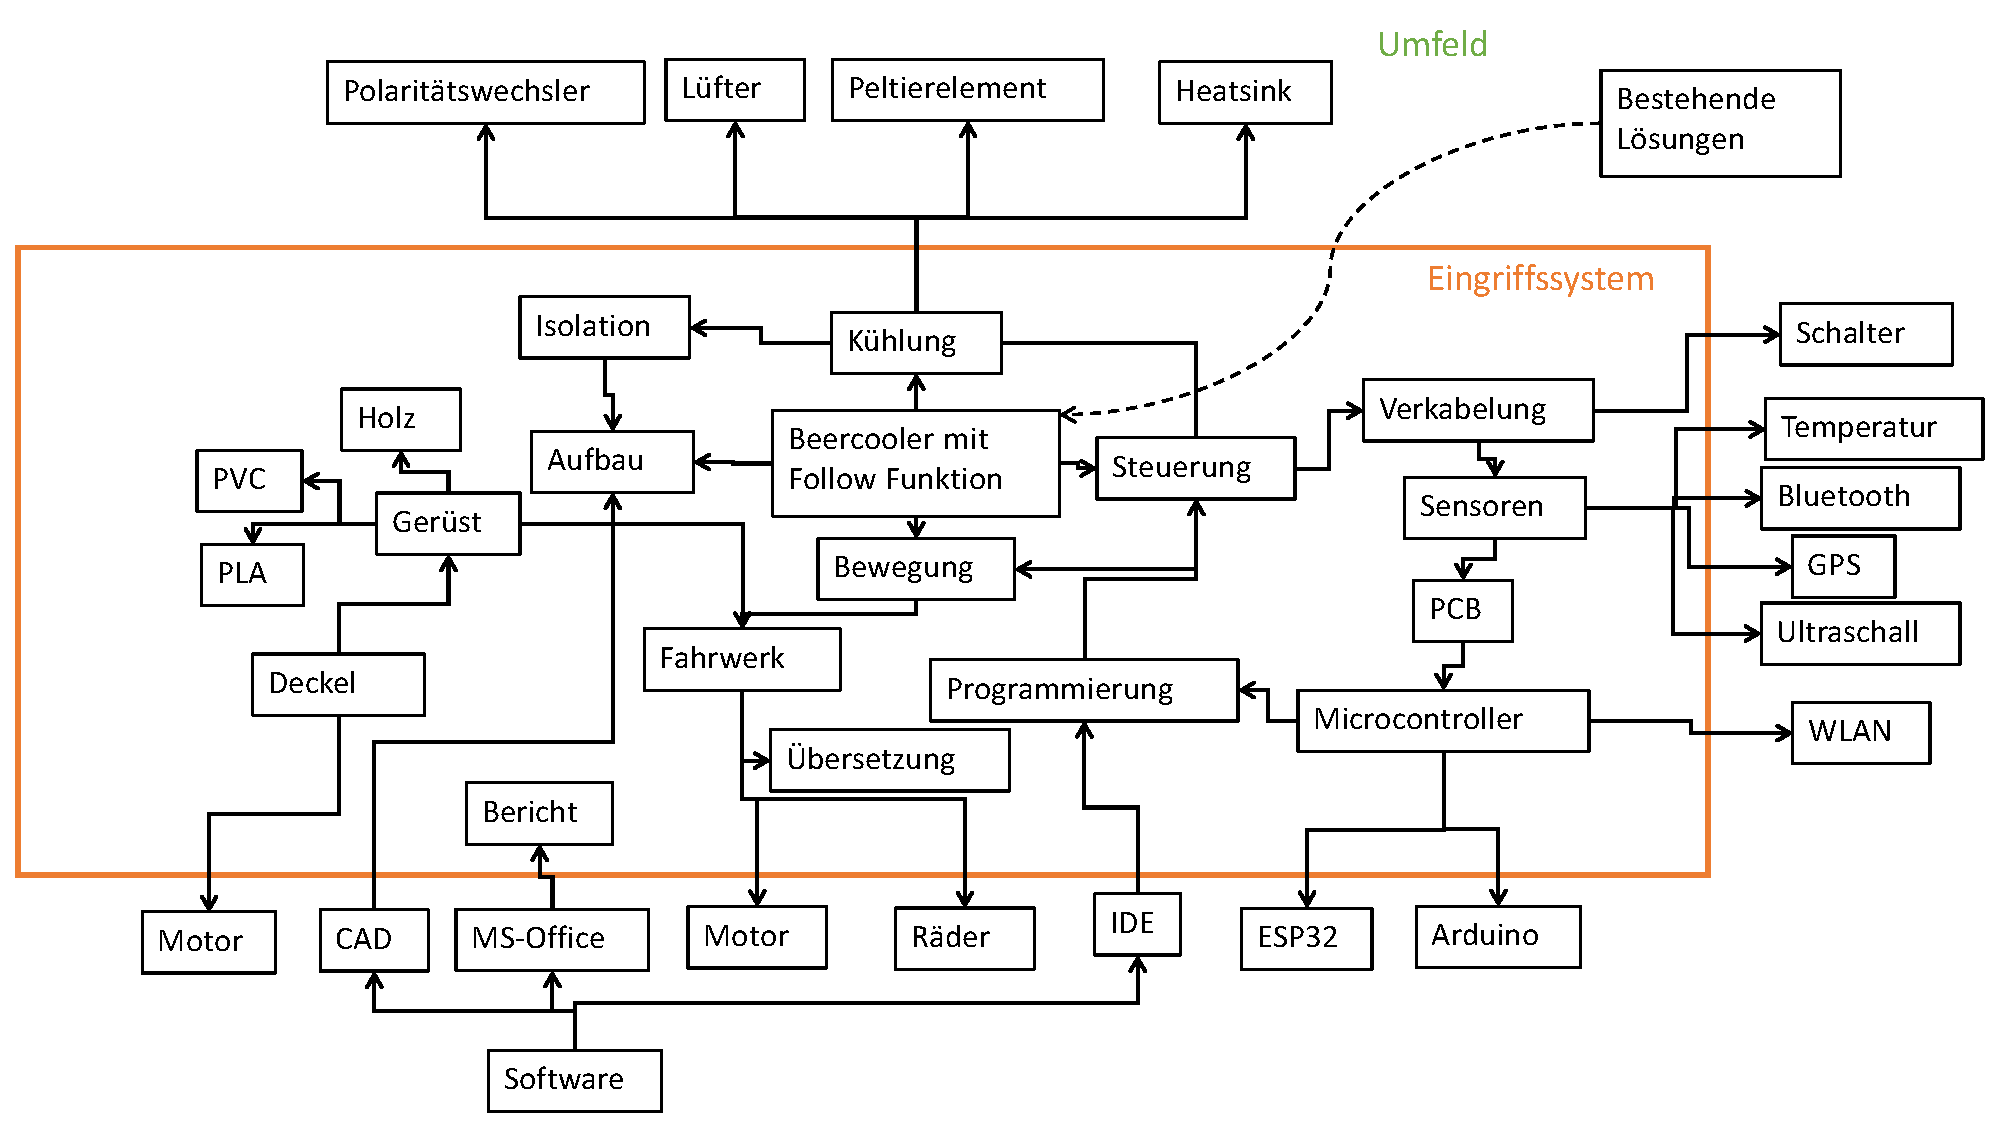
\includegraphics[width=\linewidth]{systemabgrenzung.pdf}
    \end{center}
    \caption{Systemabgrenzung}
    \label{fig:systemabgrenzung}
\end{figure}

Im Eingriffssystem sind alle Punkte enthalten für welche Eingriffe, Veränderungen und neue Konzepte im Rahmen der Aufgabenstellung zu erledigen sind. Das Umfeld beinhaltet die relevanten Teile für die Erarbeitung der Punkte im Eingriffssystem.

\subsection{Stärken- und Schwächenanalyse}
% Please add the following required packages to your document preamble:
% \usepackage{graphicx}
\begin{table}[H]
    \centering
    \caption{Stärken- und Schwächenanalyse}
    \resizebox{\columnwidth}{!}{%
    \begin{tabular}{|l|c|c|c|c|c|l|}
    \hline
    \textbf{Erfolgsfaktor} & \textbf{-{}-} & \textbf{-} & \textbf{0} & \textbf{+} & \textbf{+{}+} & \textbf{Begründung}                                 \\ \hline
    Arbeitszeiten          &             & X          &            &            &             & Zugang zum Labor ist eingeschränkt                  \\ \hline
    Betreuung              &             &            & X          &            &             & Nur während Laborzeiten                             \\ \hline
    Abgabetermin           &             &            &            & X          &             & Im Januar nach Ferien                               \\ \hline
    Innovation             &             &            & X          &            &             & Viele ähnliche Projekte   im Internet               \\ \hline
    Infrastruktur          &             &            &            & X          &             & Mechatronik Labor und FHNW   Werkstatt              \\ \hline
    Informatik Know-How    &             & X          &            &            &             & Kein Teammitglied aus   diesem Fachgebiet           \\ \hline
    Kommunikation          &             &            &            & X          &             & Ohne Probleme                                       \\ \hline
    Kosten                 &             &            & X          &            &             & Eher knapp                                          \\ \hline
    Materialbeschaffung    &             &            &            & X          &             & Selbstversorgung,   Abrechnung am Ende des Projekts \\ \hline
    Motivation             &             &            &            &            & X           & Sehr hoch, da eigen   ausgewähltes Projekt          \\ \hline
    Projekterfahrung       &             &            &            & X          &             & Nach Semester 4 und Stage   2 vorhanden             \\ \hline
    Sicherheit             &             &            & X          &            &             & LiPo Akku                                           \\ \hline
    Technisches Know-How   &             &            &            & X          &             & Unterschiedliche Stärken   der Teammitglieder       \\ \hline
    Zusammenarbeit         &             &            &            &            & X           & Sehr gut privat   befreundet                 \\ \hline
    \end{tabular}%
    }
    \label{tab:StaerkenSchwaechenAnalyse}
    \end{table}